\chapter{Результаты и их обсуждение}
\label{ch:results}

\section{Экспериментальная установка}

Чтобы определить показатель адиабаты $\gamma$, исследовалась зависимость отношения перепадов давления $\frac{\Delta p_1}{\Delta p_2}$ от времени $\tau$. Для этого применялась установка, изображённая на рис. 1. Экспериментальная установка состояла из газгольдера с углекислым газом, резиновой груши для создания избыточного давления, жидкостного манометра для измерения изменения давления в сосуде. Также имелся кран К2, соединяющий сосуд с газом с окружающей средой для исследования адиабатического расширения и изобарического нагревания газа.

\begin{figure}[ht]
\centering
    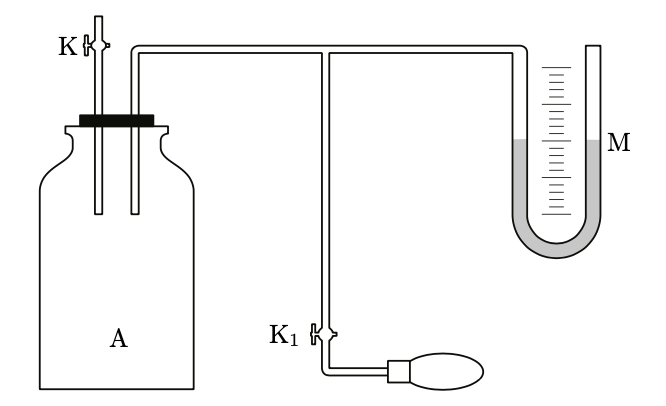
\includegraphics[width = 0.8\textwidth]{img/ust .jpg}
    \begin{center}
    Рис. 1. Экспериментальная установка для нахождения отношения $C_p/C_u$. Экспериментальная установка состояла из газгольдера с углекислым газом, резиновой груши для создания избыточного давления, жидкостного манометра для измерения изменения давления в сосуде. Также имелся кран К2, соединяющий сосуд с газом с окружающей средой для исследования адиабатического расширения и изобарического нагревания газа.  %(полностью описание) для чего, что на рисунке
    \end{center}
\end{figure}
\newpage

\section{Обработка результатов измерений}

Для определения показателя адиабаты $\gamma$ исследовали зависимость отношения перепадов давления $\frac{\Delta p_1}{\Delta p_2}$ от времени $\tau$. Давления $p_1$ и $p_2$ определялись жидкостным манометром, а их отношение равно отношению $\Delta h_1$ к $\Delta h_2$. Результаты измерений зависимости $\Delta h_1$ и $\Delta h_2$ от $\tau$ приведены в Приложении Б. 

Значение $ln(\gamma / \gamma - 1)$ можно найти по графику зависимости $\ln(\Delta h_1/\Delta h_2)$ от $\tau$, а из него просто выражается искомый показатель адиабаты $\gamma$. По данным из таблицы 1 (см. Приложение Б.) построили график зависимости $\ln(\Delta h_1/\Delta h_2)$ от $\tau$.

\begin{figure}[ht]
\centering
    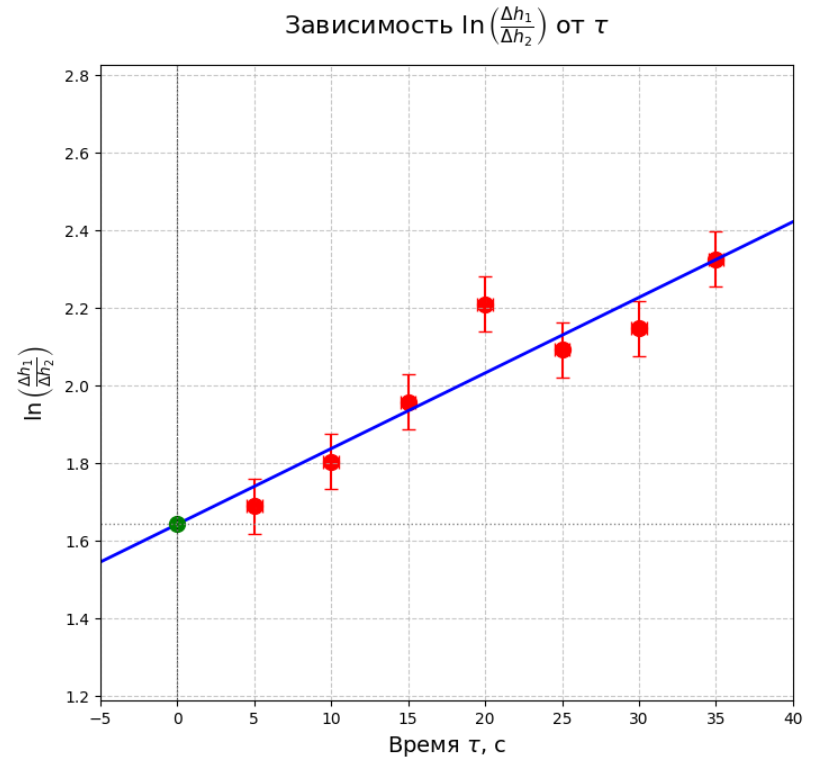
\includegraphics[width = 0.8\textwidth]{img/Ln(h1h2)(t).png}
    \begin{center}
    Рис. 2. График зависимости $ln(\Delta h_1 / \Delta h_2) (\tau)$. Красные точки - экспериментальные данные, синия линия проведена, чтобы визуально показать аппроксимацию и пересечение с прямой $\tau = 0$. Зелёная точка на графике - значение $ln(\gamma / \gamma - 1) = 1.64 \pm 0.06$, из которого определялось значение $\gamma$.  %(полностью описание) для чего, что на рисунке
    \end{center}
\end{figure}
\newpage

По графику видно, что зависимость $ln(\Delta h_1 / \Delta h_2)$ от $\tau$ линейная, это подтверждает справедливость полученной формулы для расчёта $ln(\Delta h_1 / \Delta h_2)$.Значение $ln(\gamma / \gamma - 1)$ из графика получилось равным $1.64 \pm 0.06$. Отсюда коэффициент адиабаты для углекислого газа получился равным $\gamma = 1.293 \pm 0.018$. Значение с учётом погрешности совпало с табличным  $\gamma_\text{табл} = 1.31$ \cite{Lab}. Следовательно, предложенный метод позволяет с точностью 1.5\% определить показатель адиабаты для углекислого газа. %ссылка на источник